\documentclass[10pt]{beamer}

\mode<presentation> {

% \usetheme{Berlin}  % Squares
\usetheme{Madrid}  % Circles & dense
% \usetheme{Frankfurt}  % Cirles

\setbeamertemplate{headline}{%
\leavevmode%
  \hbox{%
    \begin{beamercolorbox}[wd=\paperwidth,ht=2.5ex,dp=1.125ex]{palette quaternary}%
    \insertsectionnavigationhorizontal{\paperwidth}{}{\hskip0pt plus1filll}
    \end{beamercolorbox}%
  }
}

\setbeamertemplate{navigation symbols}{}  % To remove the navigation symbols from the bottom of all slides uncomment this line

% \useoutertheme{miniframes}
% \useinnertheme{circles}

}

\usepackage{graphicx}
\usepackage{booktabs}
\usepackage{fontspec}
\usepackage{xunicode}
\usepackage{xltxtra}
\usepackage{xecyr}
\usepackage{hyperref}
\usepackage{amsthm}
\usepackage{blindtext}

\usepackage{polyglossia}
\setdefaultlanguage{russian}
\setmainfont[Mapping=tex-text]{CMU Serif}
\setsansfont[Mapping=tex-text]{CMU Sans Serif}
\setmonofont[Mapping=tex-text]{CMU Serif}

\makeatletter
\DeclareUrlCommand\ULurl@@{%
  \def\UrlFont{\ttfamily\color{blue}}%
  \def\UrlLeft{\uline\bgroup}%
  \def\UrlRight{\egroup}}
\def\ULurl@#1{\hyper@linkurl{\ULurl@@{#1}}{#1}}
\DeclareRobustCommand*\ULurl{\hyper@normalise\ULurl@}
\makeatother

\newcommand\TODO[1]{\textcolor{red}{{\Large TODO: #1}}}
\newcommand\NaN{\textcolor{red}{NaN}}
\newcommand{\X}[1]{X_{\texttt{#1}}}
\newcommand{\Xaux}{\X{aux}}
\newcommand{\Xdata}{\X{data}}
\newcommand{\Xtrain}{\X{train}}
\newcommand{\Xtest}{\X{test}}
\newcommand{\Xgen}{\X{gen}}
%-------------------------------------------------------------------------------
%	TITLE PAGE
%-------------------------------------------------------------------------------
\title[Управляемая генерация текста]{Управляемая генерация текста c использованием механизма внимания%Controllable text generation with small data using auxiliary in-domain enrichment
}
\author[Беляев Станислав]{
Беляев Станислав\texorpdfstring{\\ Научный руководитель: Николенко Сергей Игоревич}{}
}
\institute[СПбАУ]
{
Санкт-Петербургский Академический Университет \\
\medskip
\textit{stasbelyaev96@gmail.com}
}
\date{25 мая 2018}
\begin{document}
%-------------------------------------------------------------------------------
%	PRESENTATION SLIDES
%-------------------------------------------------------------------------------
\begin{frame}
\titlepage
\end{frame}
%-------------------------------------------------------------------------------
\section{Введение}
\begin{frame}
\frametitle{Введение}
\framesubtitle{Постановка задачи}

\begin{center}
    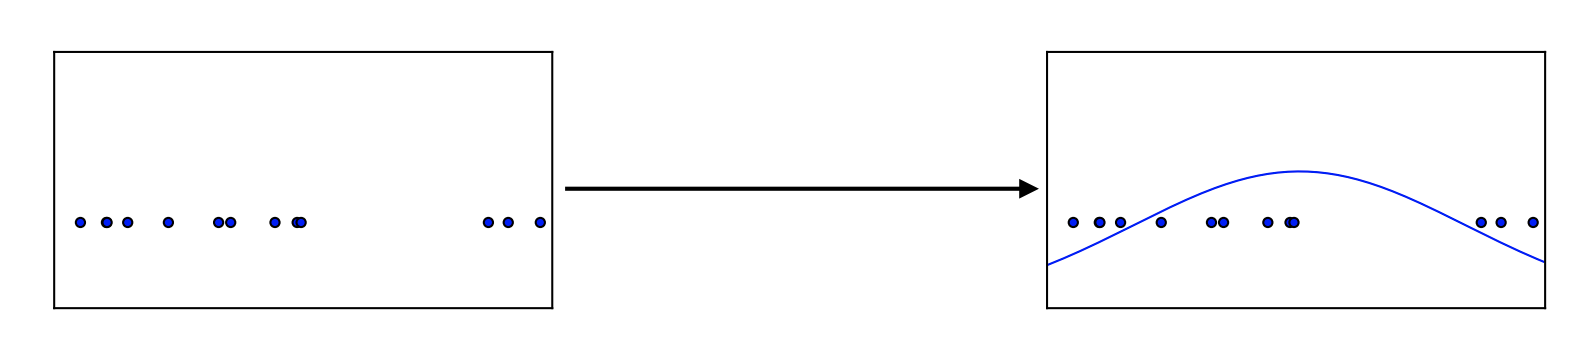
\includegraphics[height=2cm]{images/density_estimation.png}\\
    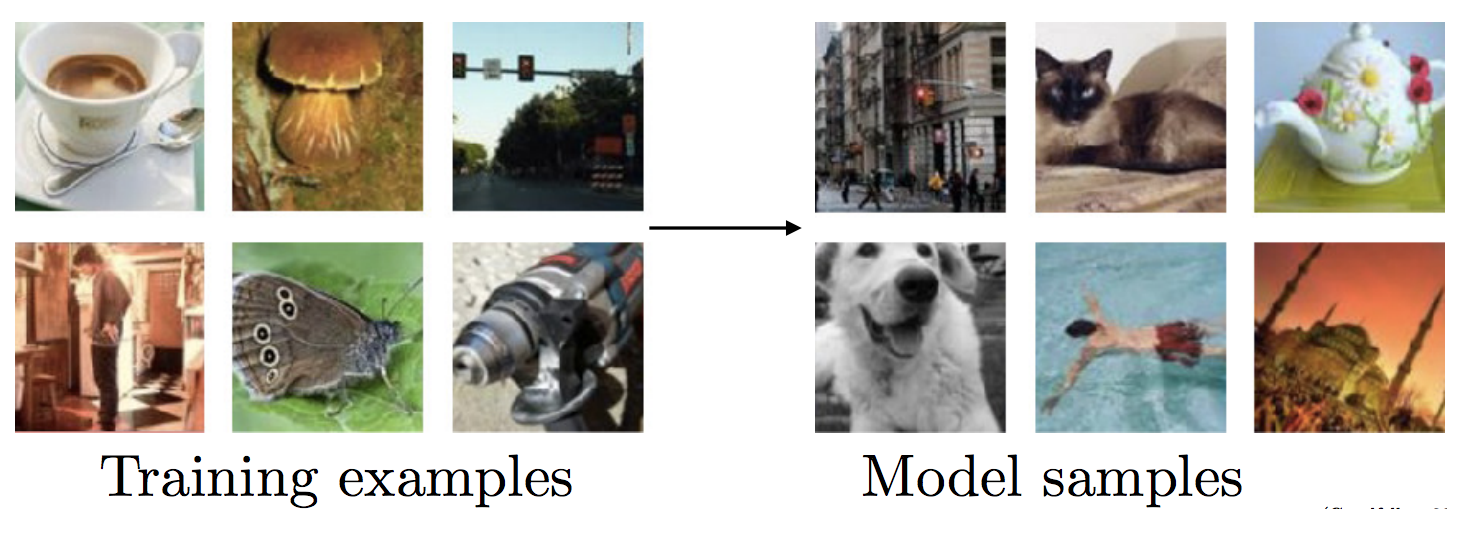
\includegraphics[height=3cm]{images/density_samples.png}
\end{center}

\underline{Задача}: Построить $p_{\texttt{model}}(x)$, моделирующее $p_{\texttt{data}}(x)$ по набору данных $x \in X_{\texttt{train}}$ из генеральной совокупности $X$, содержащей некий набор свойств $f = \{f_i \in F\}$. \\
Возьмем в качестве $X$ текст общего характера с частично размеченными свойствами (время, окраска). % Просто потому-что, это наиболее часто встречаемый текст в реальном мире.

\end{frame}
%-------------------------------------------------------------------------------
\begin{frame}
\frametitle{Введение}
\framesubtitle{Особенности}

Актуальность (Goodfellow et al., 2017):
\begin{itemize}
    \item Универсальная статистическая задача для многомерных данных
    \item Применения в RL для генерации событий окружения (Finn et al., 2016)
    \item Обучение с частичной разметкой (Semi-supervised) и с пропусками в данных
    \item Частичная помощь или замена человека в задачах генерации (MOOC, юмор, искусство)
\end{itemize}

Сложность:
\begin{itemize}
    \item Оценка генерации (данные и метрики)
    \item Частичная и неполная разметка, не все свойства присутствуют явно
    \item Сложные данные редко хорошо обобщаются
    \item Поддерживать одновременно связность, правдоподобность и разнообразие
\end{itemize}

\end{frame}
%-------------------------------------------------------------------------------
\begin{frame}
\frametitle{Введение}
\framesubtitle{Изображения vs текст}

\begin{columns}[T]
    \begin{column}[T]{0.5\textwidth}
        \begin{center}
            Изображения \\
            
\includegraphics[width=0.5\textwidth]{images/image_as_func.png} \\
            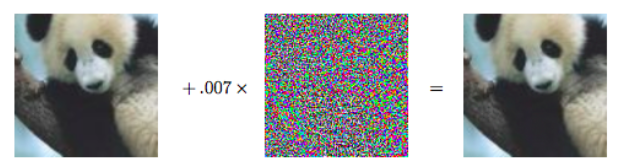
\includegraphics[width=\textwidth]{images/panda_plus_noise.png} \\
            \begin{itemize}
                \item Непрерывное пространство
                \item Набор всевозможных преобразований как дифференцируемых функций
                \item Понятно, куда распространять градиент
            \end{itemize}
        \end{center}
    \end{column}
    \vline
    \begin{column}[T]{0.5\textwidth}
        \begin{center}
            Текст \\
            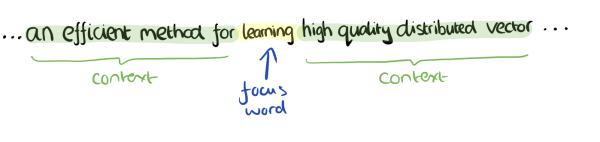
\includegraphics[width=0.9\textwidth]{images/word_context.png} \\
            \begin{itemize}
                \item Дискретное пространство
                \item Переменная длинна
                \item Нет устойчивости к шуму
                \item Long-term зависимости
                \item Омонимия и контекст
            \end{itemize}
        \end{center}
    \end{column}
\end{columns}

\end{frame}
%-------------------------------------------------------------------------------
\section{Данные}
\begin{frame}
\frametitle{Данные}
\framesubtitle{Проблема данных}

Если мы не знаем паттерна для генерации и хотим уметь обощать, то нужно больше данных и DL (Mikolov et al., 2010). \\

\begin{columns}
    \begin{column}{0.5\textwidth}
        \vskip2mm
        Но что делать, если данных мало?
        \begin{itemize}
            \item Мы не сможем обобщать 
            \item Мы скорее всего переобучимся
            \item При генерации новые сэмплы будут слишком похожи на старые
            \item Мы не сможем выучить свойства
        \end{itemize}
        Датасеты:
        \begin{itemize}
            \item \textbf{IMDB}, \textbf{SST}, Lexicon, 20NEWS
            \item Условия задачек $|X_{\texttt{task}}| = 750k$ с частичной разметкой
            \item SMILES представления молекул
        \end{itemize}
    \end{column}
    \begin{column}{0.5\textwidth}
        \begin{center}
            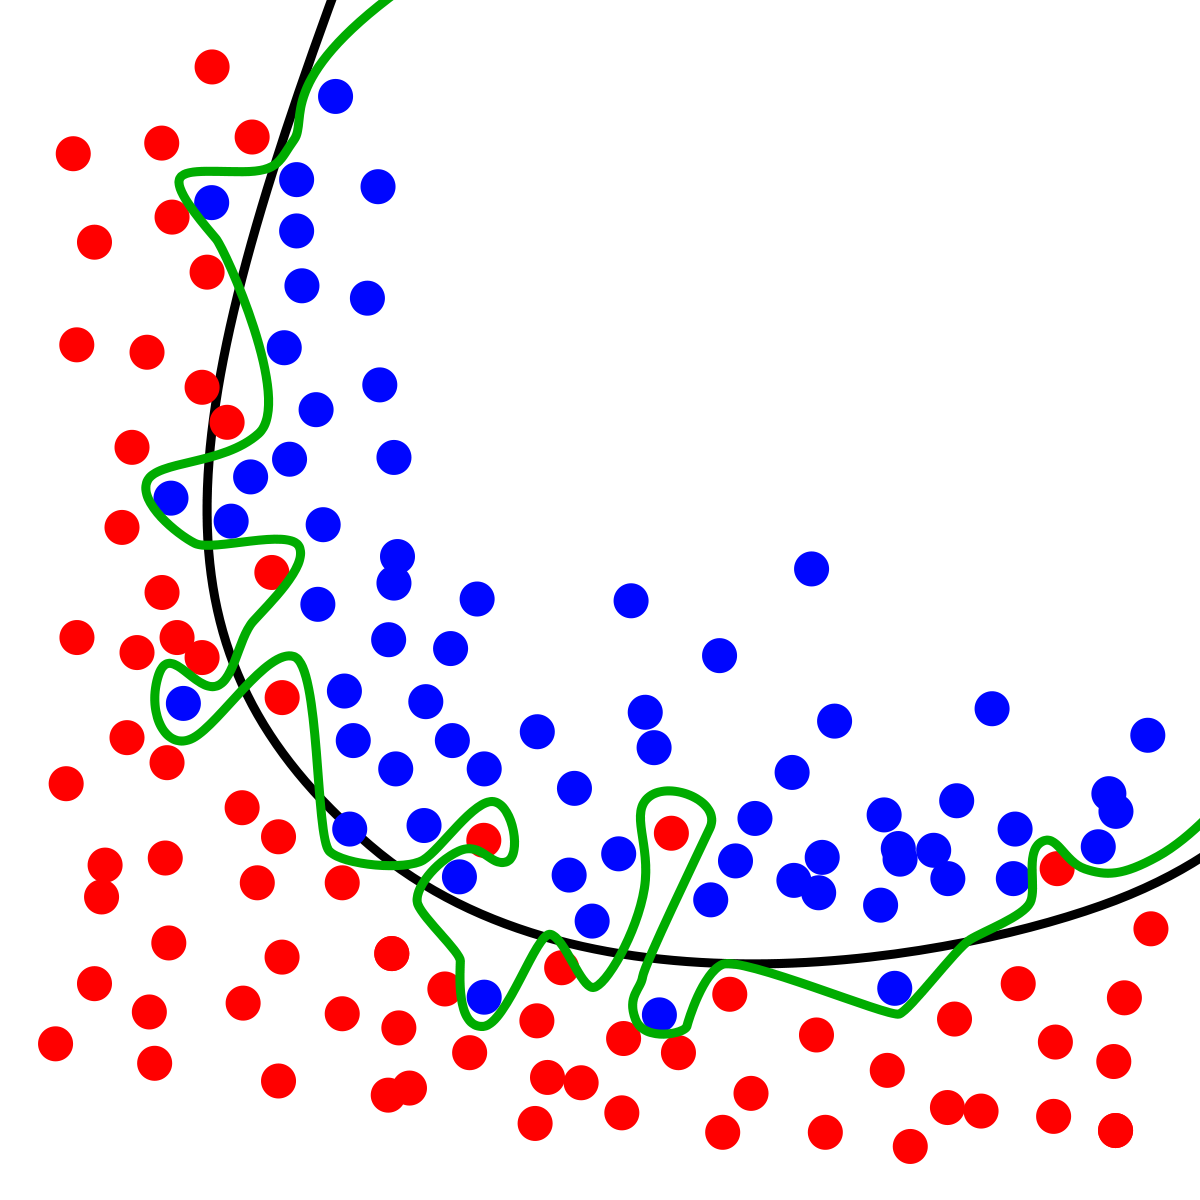
\includegraphics[width=0.7\textwidth]{images/overfitting.png}
        \end{center}
    \end{column}
\end{columns}

\underline{Решение}: Semi-supervised подходы c $X_{\texttt{aux}} \sim X$ in-domain данных из смежных областей.

\end{frame}
%-------------------------------------------------------------------------------
\section{Генерация}
\begin{frame}
\frametitle{Генерация}
\framesubtitle{Метрики}

Как можно оценить результат генерации? (Salimans et al., 16)
\begin{itemize}
    \item Автоматические метрики для $W \in \Xtest$ и новых сэмлов $W \in \Xgen$
    \begin{block}{Perplexity}
        $PP(W) = P(w_1w_2w_3\dots w_{|W|})^{-\frac{1}{|W|}} = \left[\prod\limits_{i=1}^{|W|}{\frac{1}{P(w_i|w_1\dots w_{i-1})}}\right]^{\frac{1}{|W|}}$
    \end{block}
    \begin{block}{BLEU, Self-BLEU}
        BLEU(R, S) \in [0, 1], ~ \texttt{N-gram'ая схожесть предложений}
    \end{block}
    \item Assessors evaluation
        \begin{itemize}
            \item MTurk, Я.Толока
            \item DCG, MAP
        \end{itemize}
    \item Самому
        \begin{itemize}
            \item Generic-генерация и генерация по заданным свойствам
            \item Быстрая и дешевая проверка
        \end{itemize}
\end{itemize}

\end{frame}
%-------------------------------------------------------------------------------
\begin{frame}
\frametitle{Генерация}
\framesubtitle{Таксономия генеративных моделей}

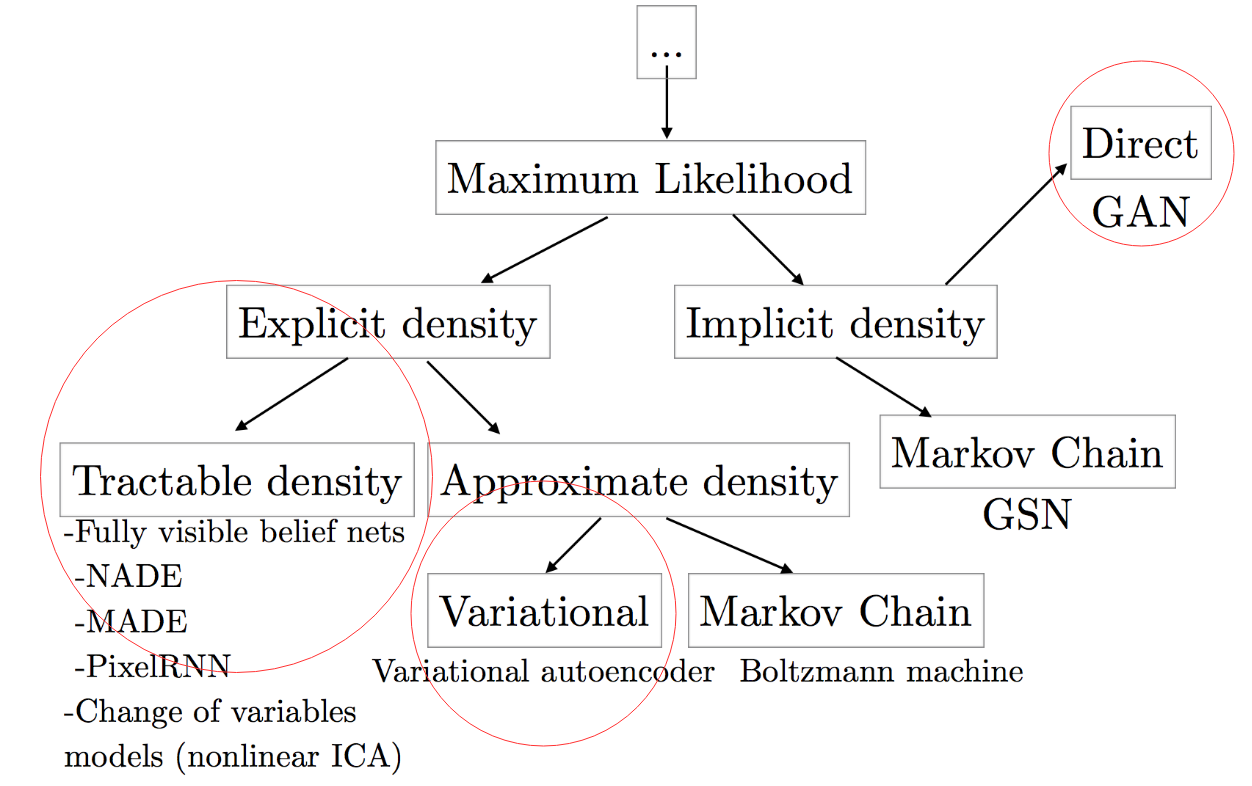
\includegraphics[width=\textwidth]{images/gen_taxonomy2.png}

\end{frame}
%-------------------------------------------------------------------------------
\section{RNN}
\begin{frame}
\frametitle{RNN}
\framesubtitle{Обзор}

\begin{center}
    \begin{column}{0.7\textwidth}
        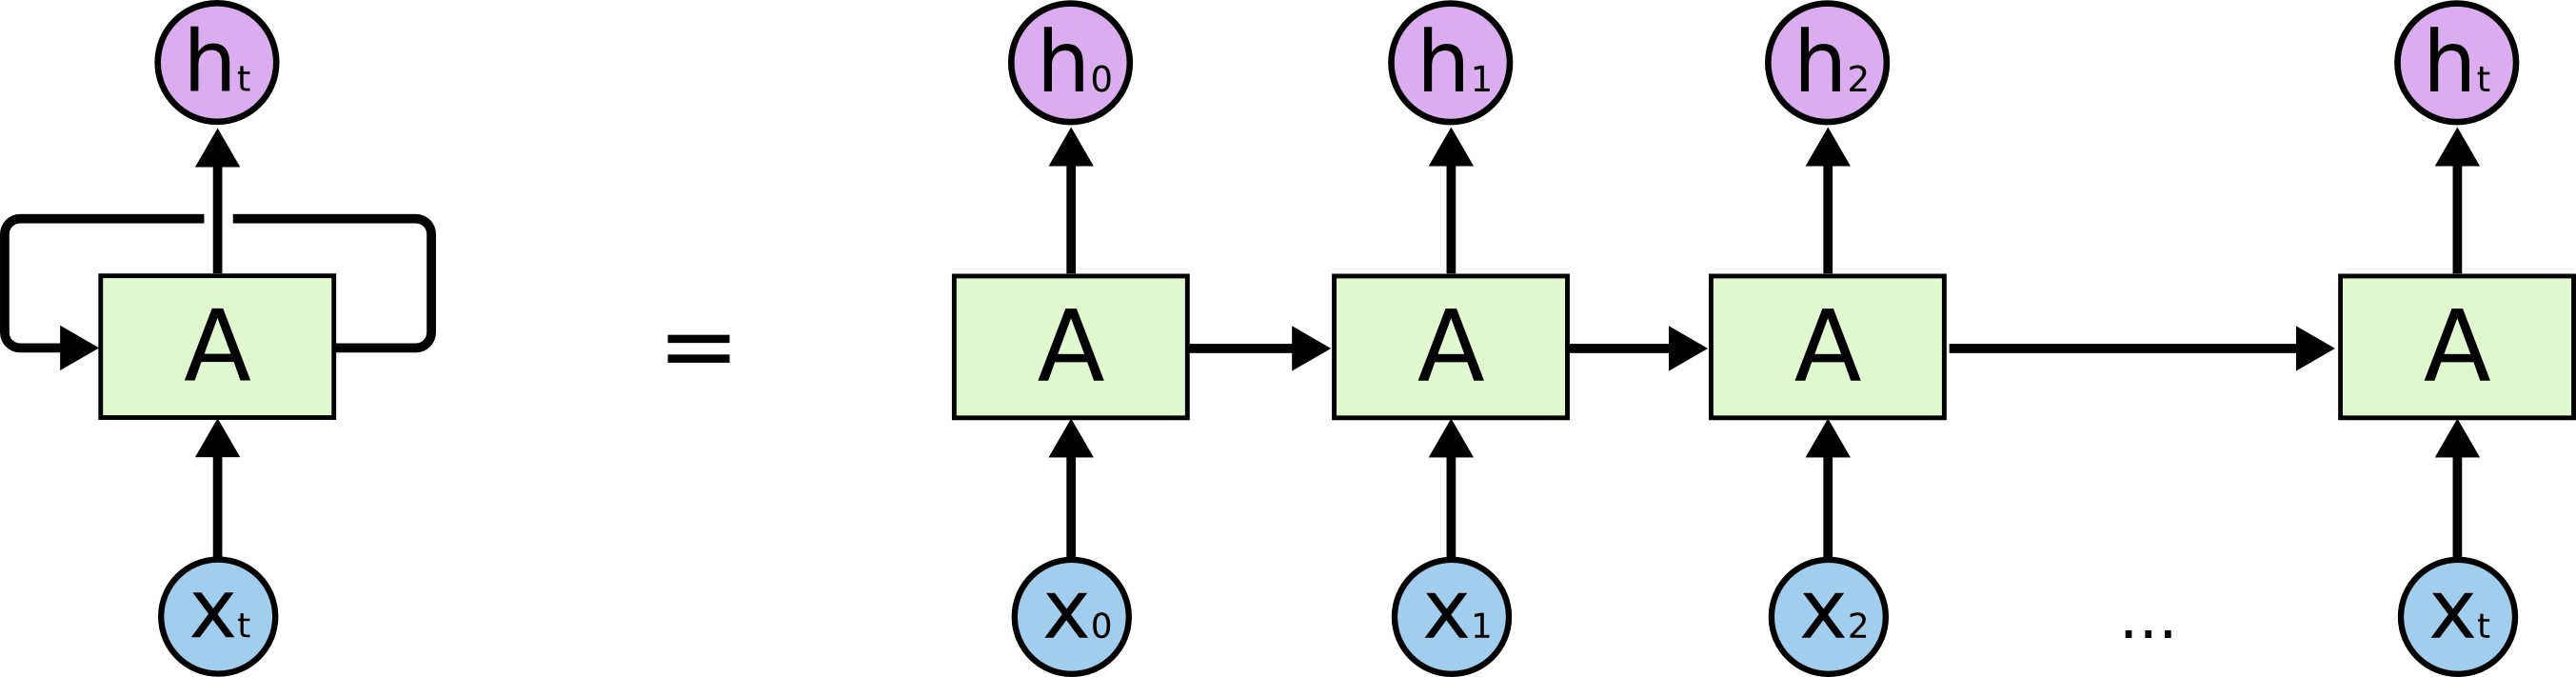
\includegraphics[height=0.25\textheight]{images/rnn_unrolled.png}
    \end{column}
    \begin{column}{0.25\textwidth}
        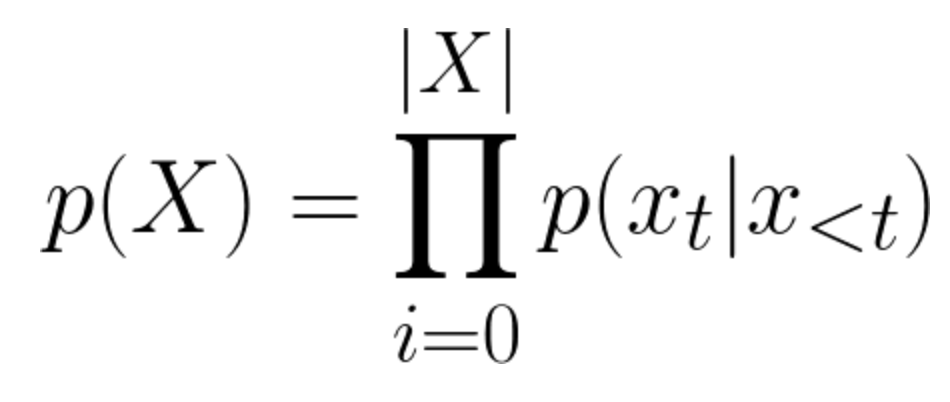
\includegraphics[height=0.14\textheight]{images/rnn_p.png}
    \end{column}
    % 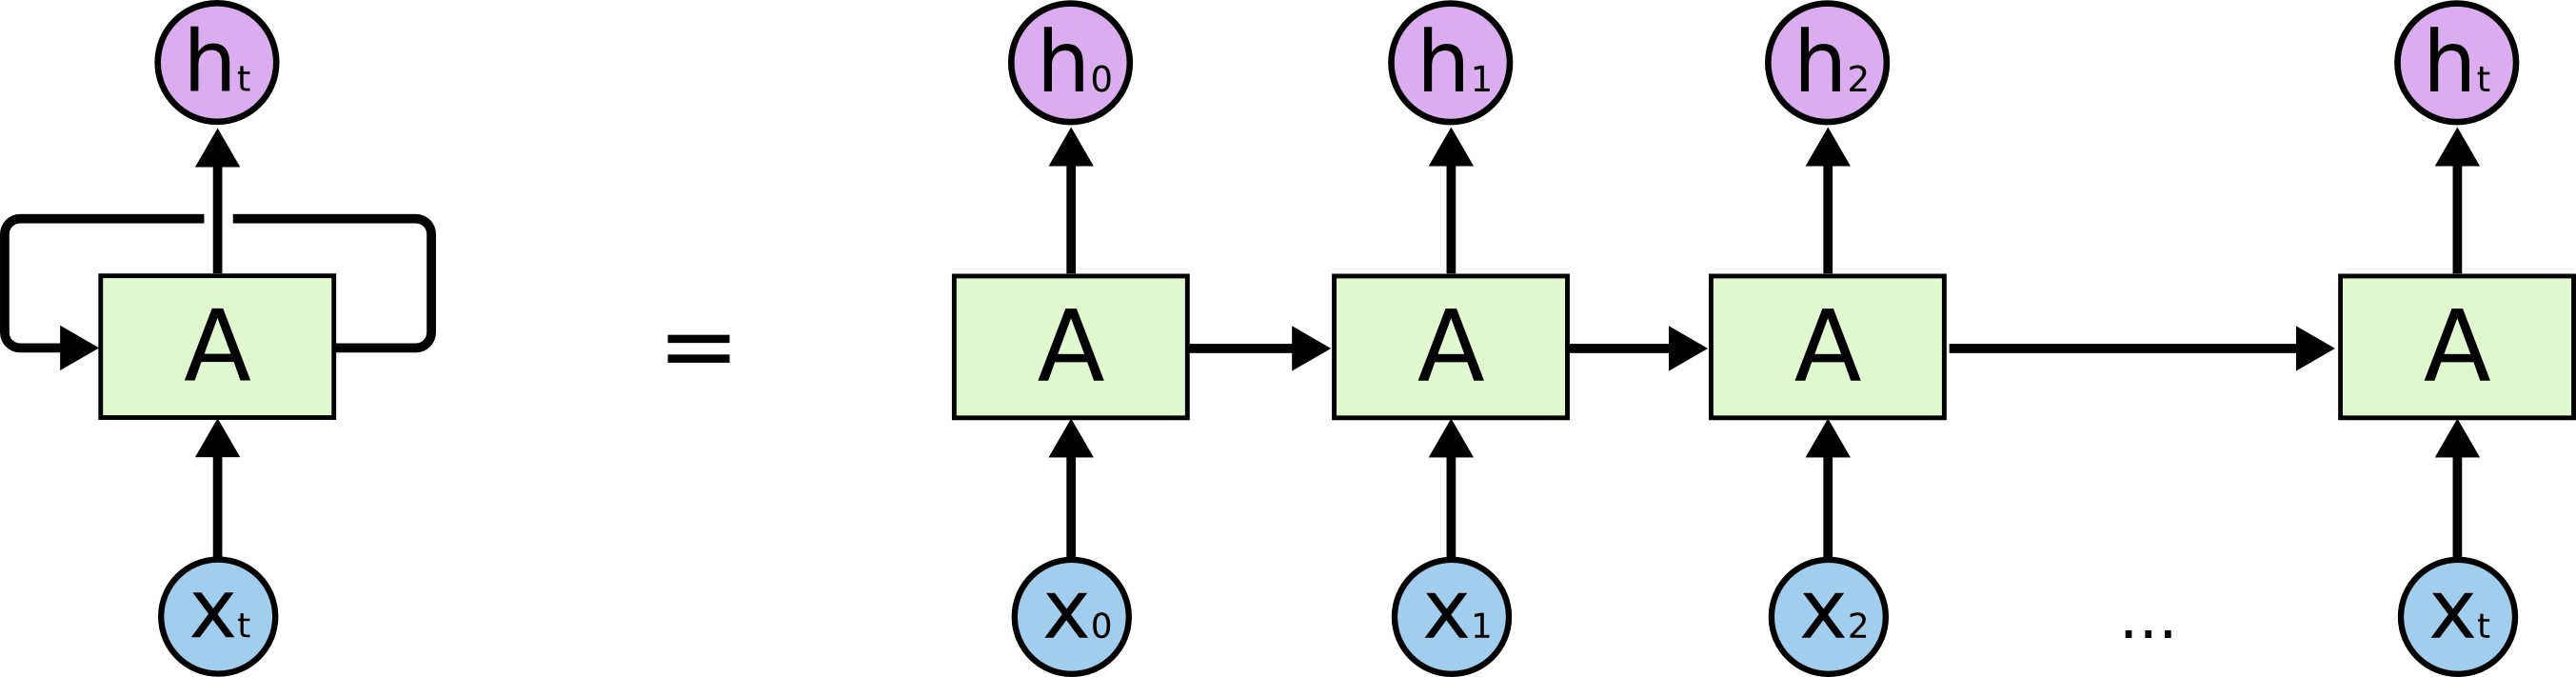
\includegraphics[height=0.25\textheight]{images/rnn_unrolled.png}\\
    \vskip2mm
    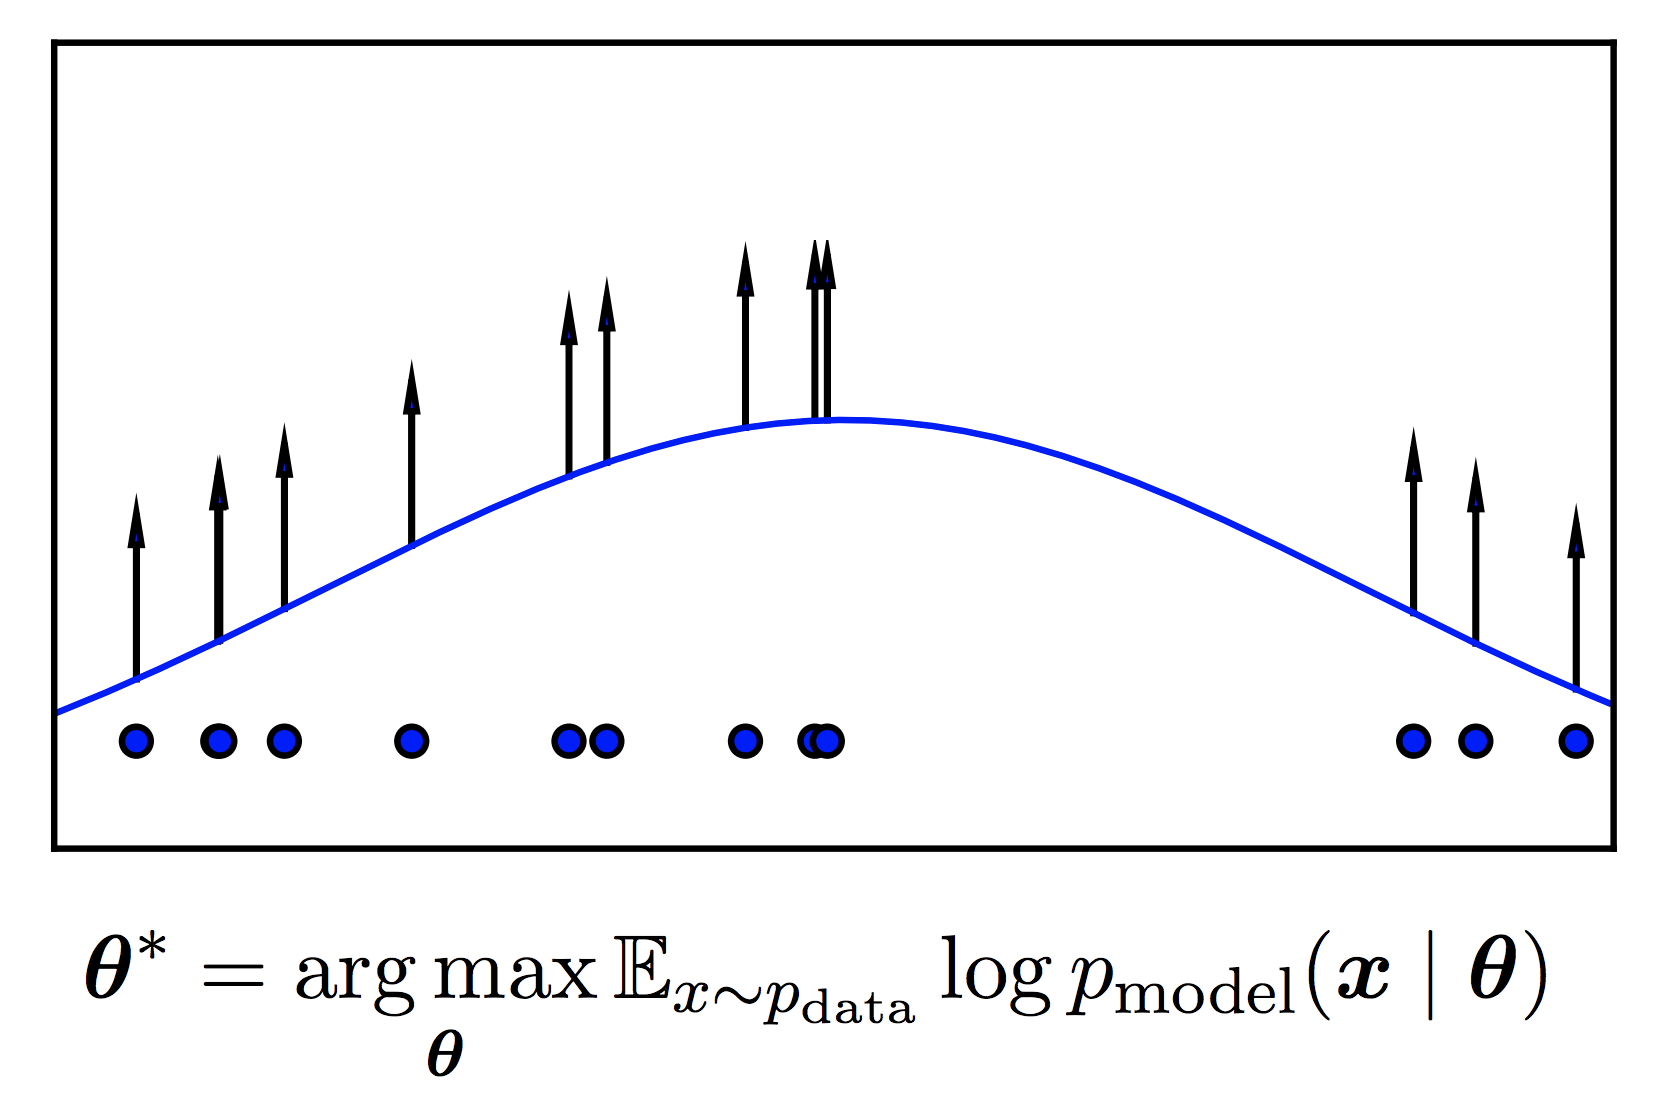
\includegraphics[height=0.5\textheight]{images/mll_density.png}
\end{center}

\end{frame}
%-------------------------------------------------------------------------------
\begin{frame}
\frametitle{RNN}
\framesubtitle{+/- (Bengio et al., 2017)}

\begin{columns}
    \begin{column}{0.5\textwidth}
        Преимущества:
        \begin{itemize}
            \item Эффективное обучение
            \item Легко реализовать и дополнить
            \begin{itemize}
                \item layers, dropout, scheduled sampling, attention, ensembling, hierachy, cnn, ...
            \end{itemize}
            \item Эффективное сэмплирование
            \begin{itemize}
                \item greedy decoding / beam search
                \item регуляризация на кандидатов
            \end{itemize}
            \item Оценка совместной вероятности cлов
        \end{itemize}
        Недостатки:
        \begin{itemize}
            \item Небольшая perplexity и связность
            \item Supervised-only
            \item Как задать начальные условия?
            \begin{itemize}
                \item out-of-band / in-band ($x \Rightarrow f + '|' + x + '|' + f$)
            \end{itemize} 
        \end{itemize}
    \end{column}
    \begin{column}{0.5\textwidth}
        \begin{center}
            \vskip-8mm
            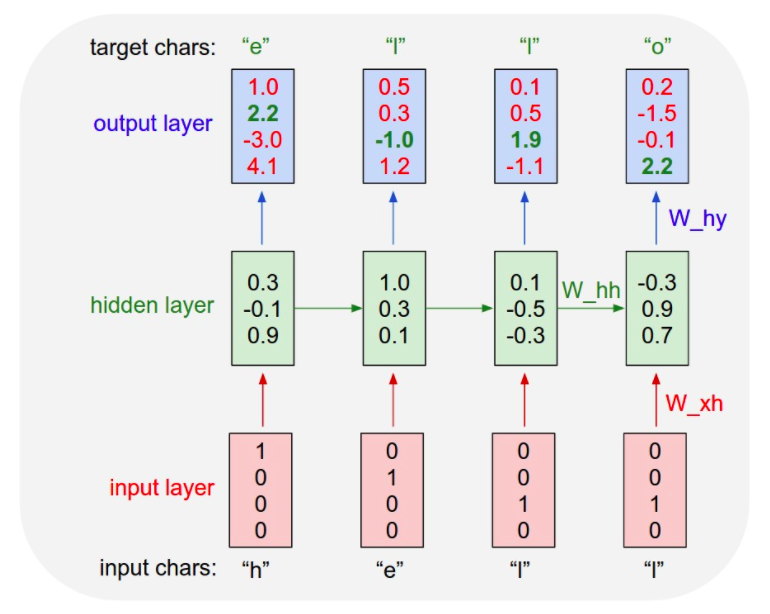
\includegraphics[width=0.7\textwidth]{images/rnn.png}\\
            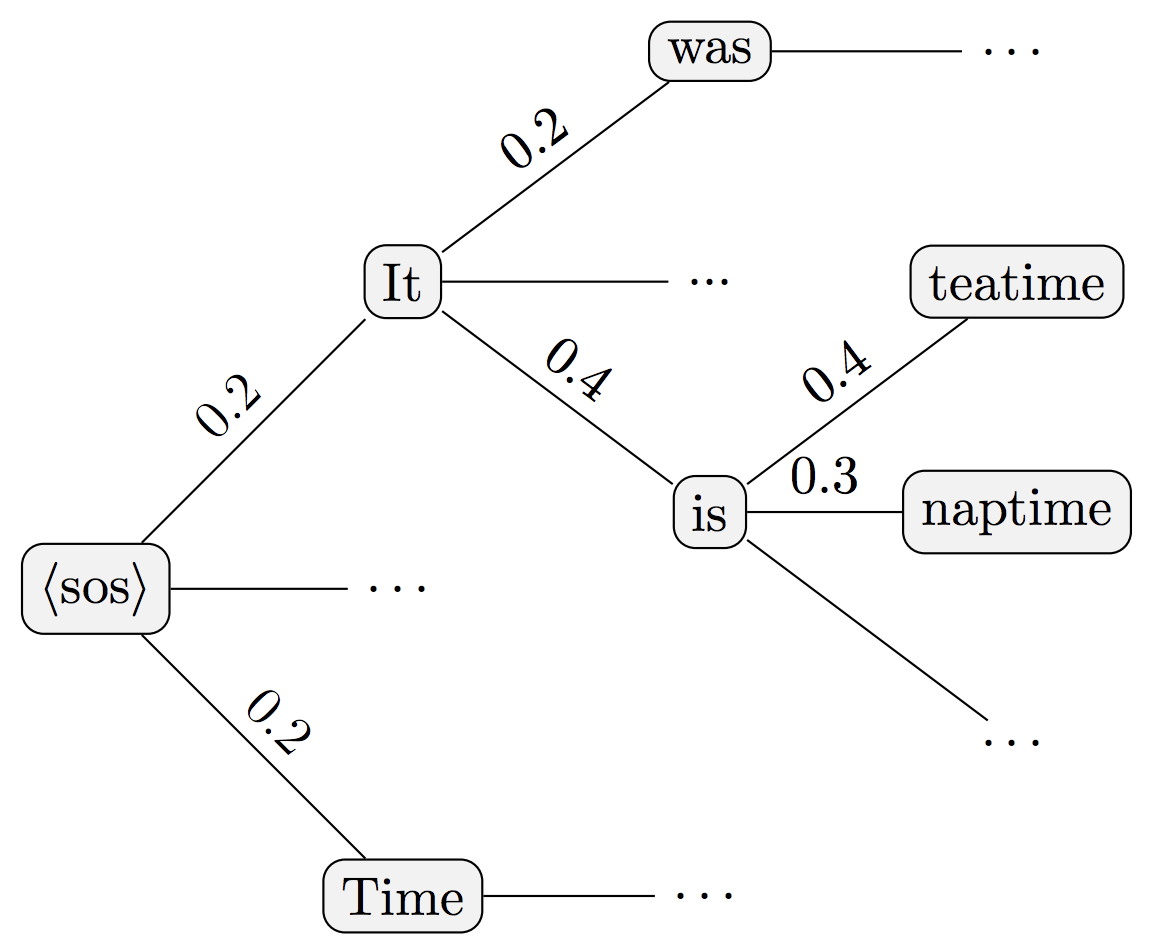
\includegraphics[width=0.7\textwidth]{images/beam_search.png}
        \end{center}
    \end{column}
\end{columns}

\end{frame}
%-------------------------------------------------------------------------------
\section{GAN}
\begin{frame}
\frametitle{GAN}
\framesubtitle{Обзор и вариации}

\begin{columns}
    \begin{column}{0.35\textwidth}
        \begin{center}
            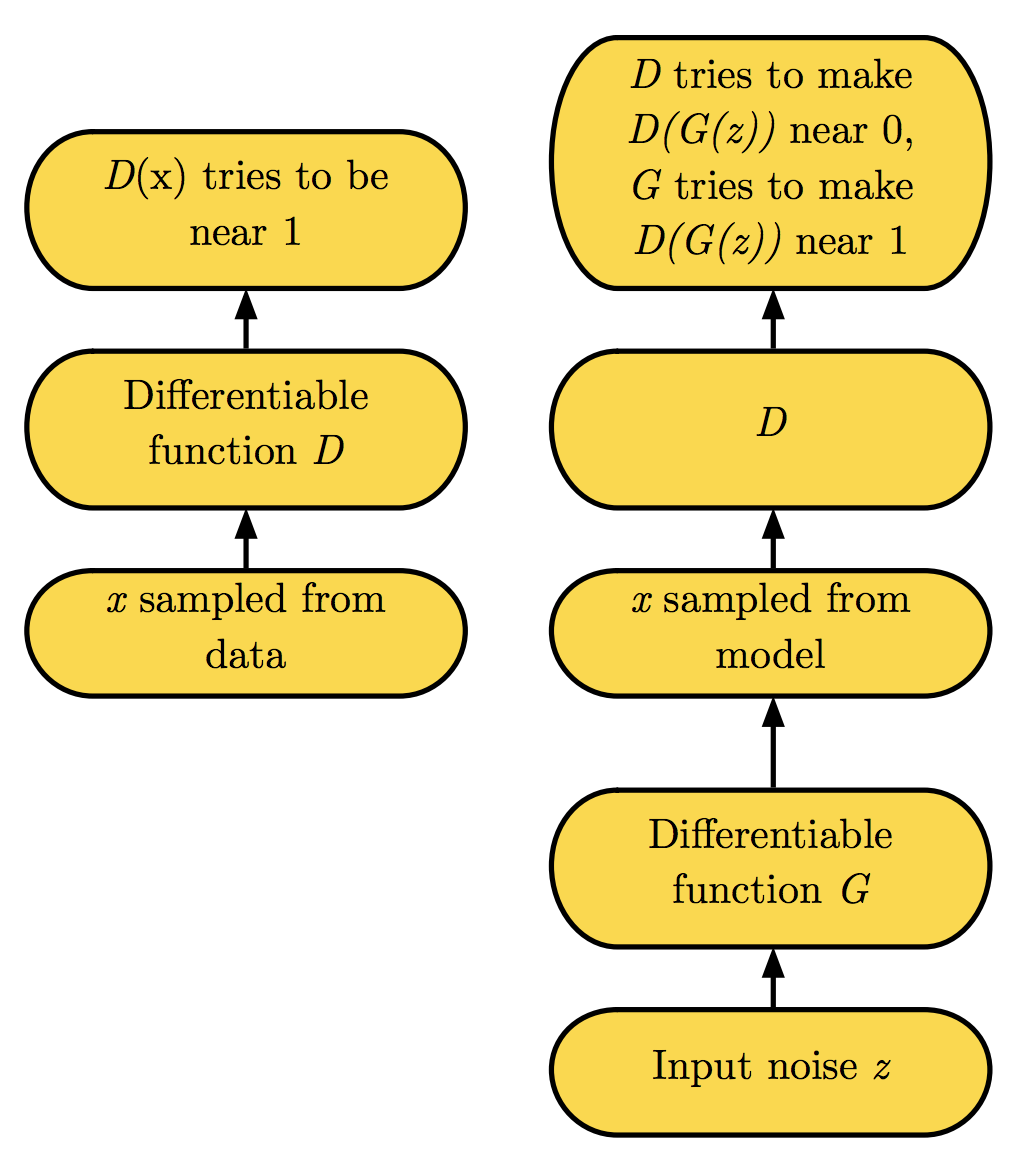
\includegraphics[width=\textwidth]{images/gan_fw.png}
        \end{center}
    \end{column}
    \begin{column}{0.65\textwidth}
        \begin{center}
            \vskip-8mm
            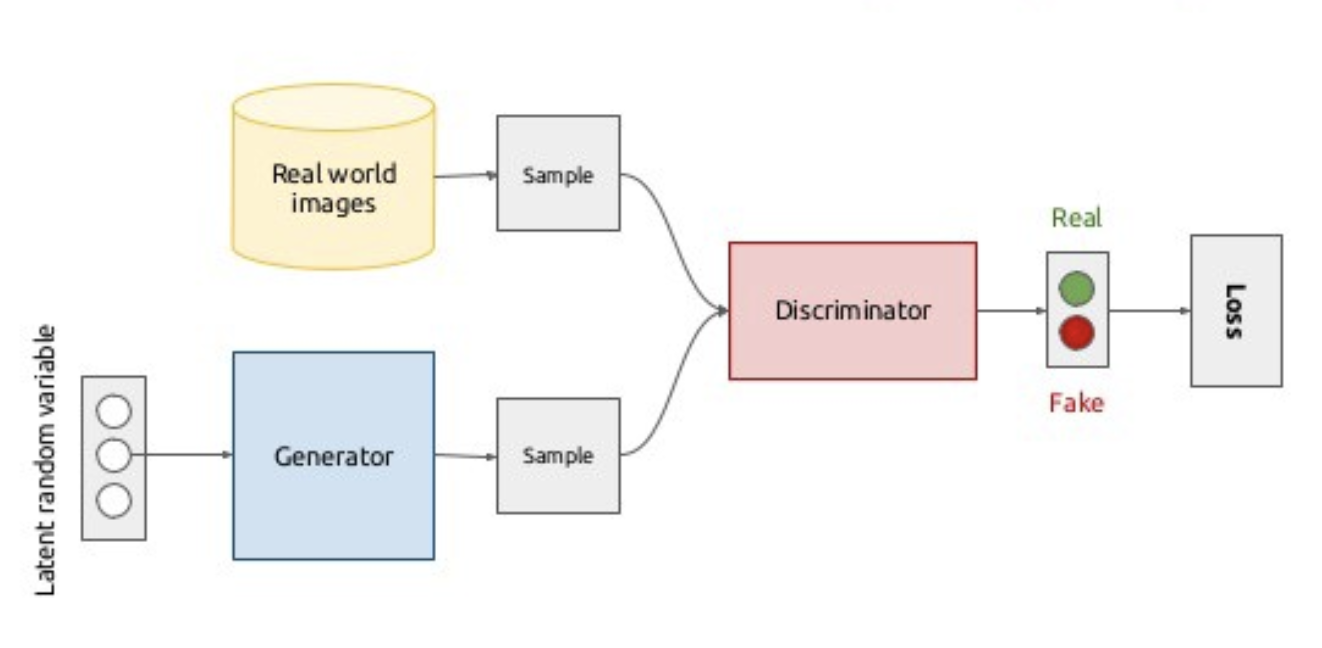
\includegraphics[width=\textwidth]{images/fan_ov.png}\\
            
\includegraphics[width=\textwidth]{images/gan_loss.png}\\
            \vskip2mm
            Для дискретных значений: (Goodfellow et al., 17)
            \begin{itemize}
                \item REINFORCE (SeqGAN, LeakGAN)
                \item GumbelSoftmax (GSGAN)
                \item Embeddings ($\mathbb{N} \Rightarrow \mathbb{R}^n$)
            \end{itemize}
        \end{center}
    \end{column}
\end{columns}

\end{frame}
%-------------------------------------------------------------------------------
\begin{frame}
\frametitle{GAN}
\framesubtitle{Результаты}

\begin{columns}
    \begin{column}{0.5\textwidth}
        \begin{center}
            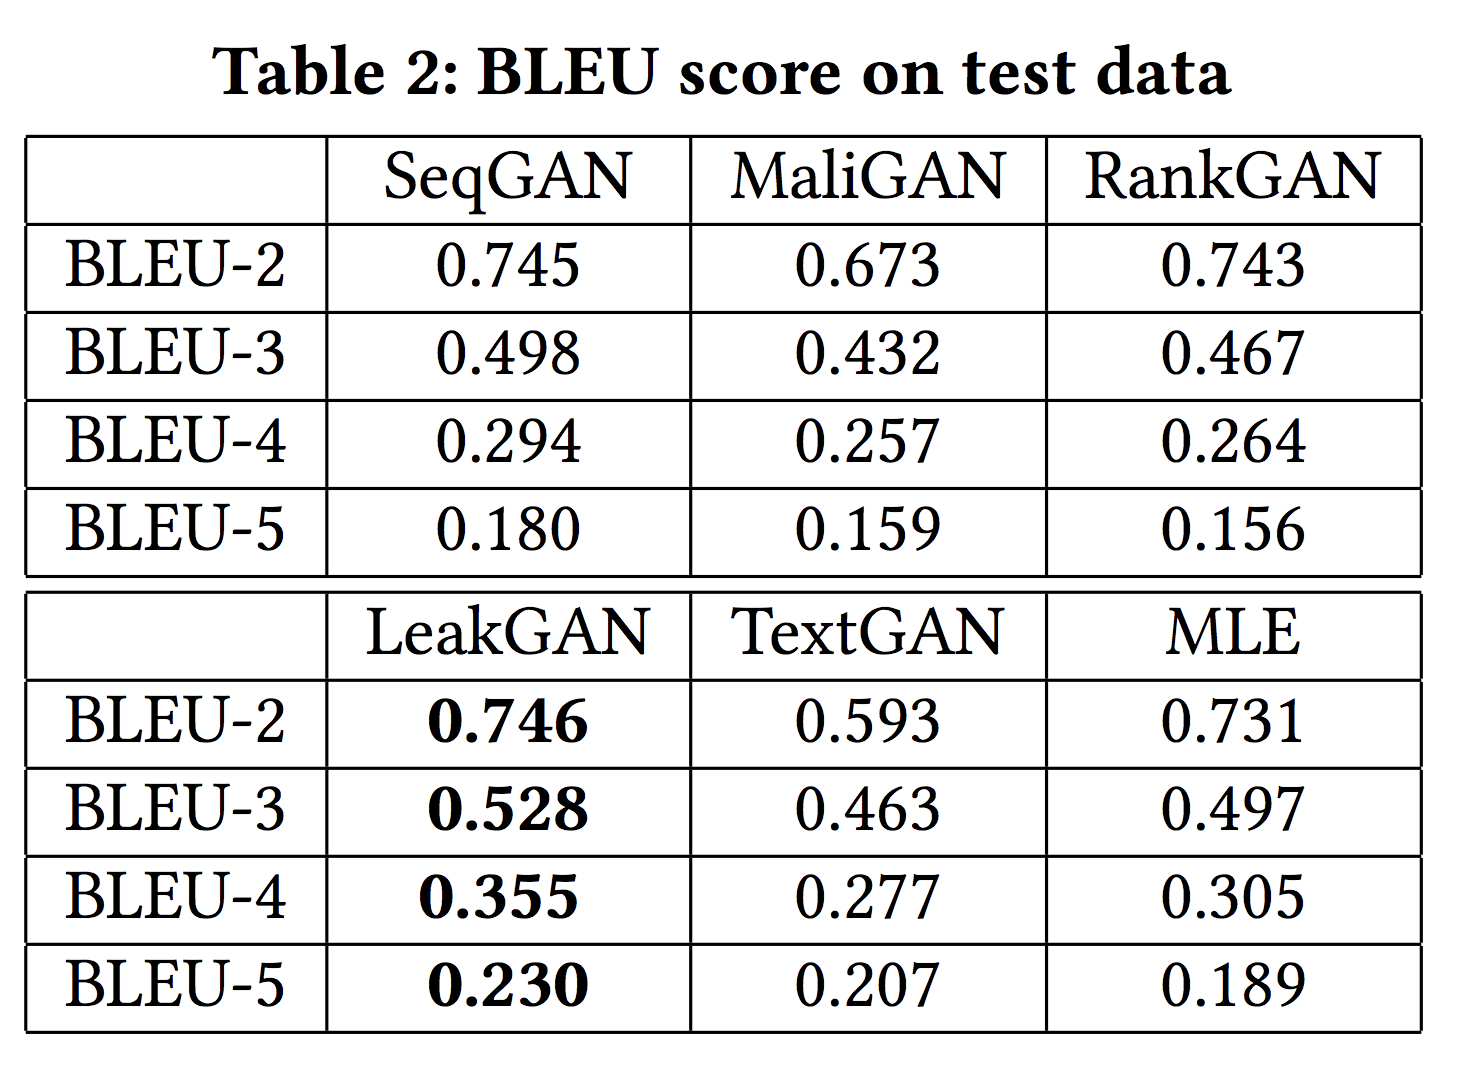
\includegraphics[width=\textwidth]{images/gan_bleu.png}
        \end{center}
    \end{column}
    \begin{column}{0.5\textwidth}
        \begin{center}
            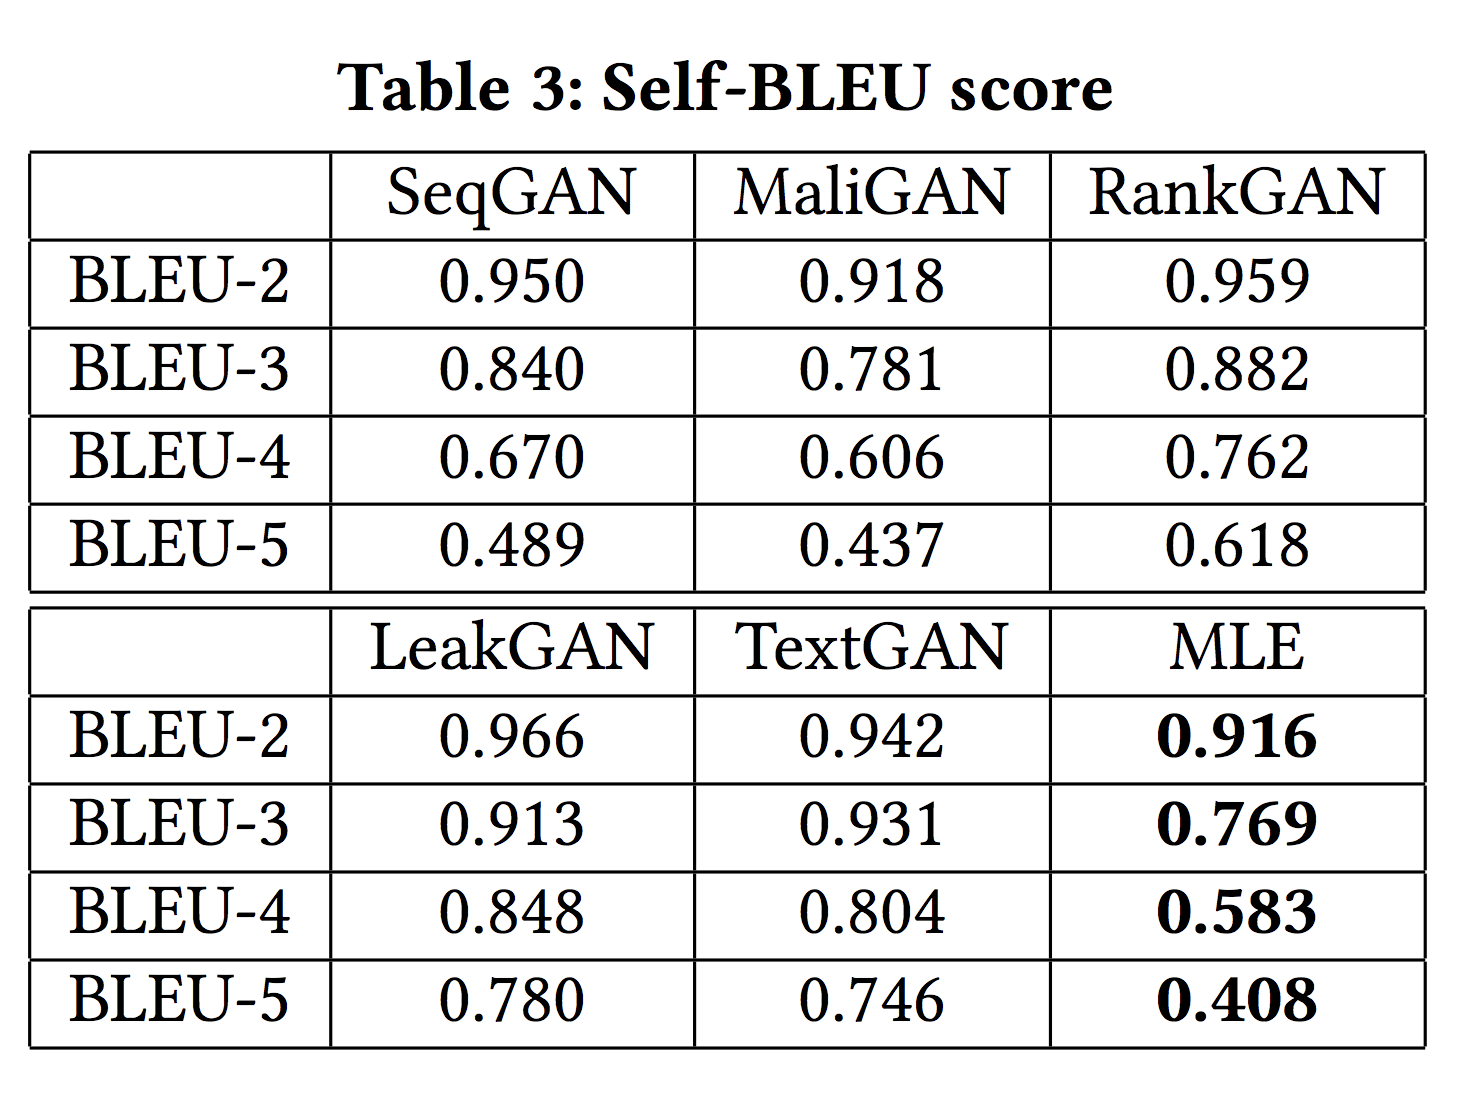
\includegraphics[width=\textwidth]{images/gan_self_bleu.png}
        \end{center}
    \end{column}
\end{columns}

\end{frame}
%-------------------------------------------------------------------------------
\begin{frame}
\frametitle{GAN}
\framesubtitle{Mode collapsing}

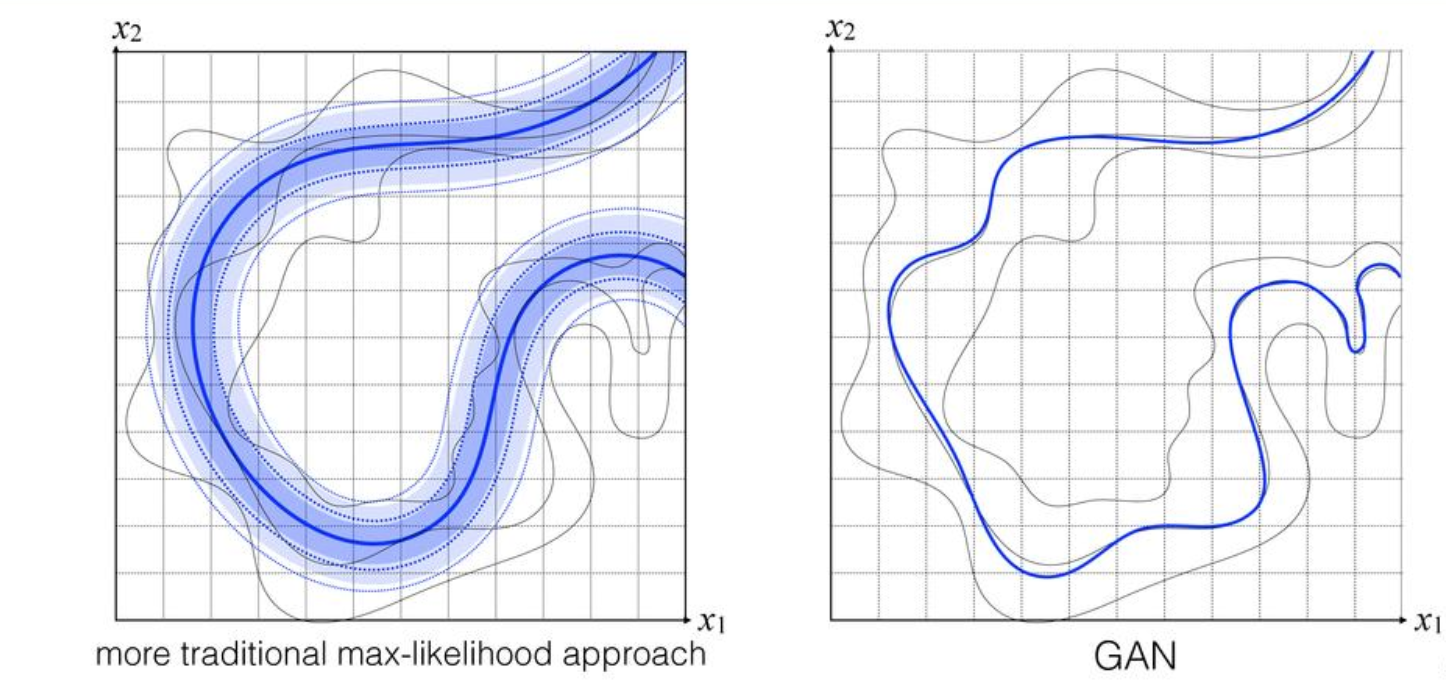
\includegraphics[width=\textwidth]{images/ml_vs_gan.png}

\end{frame}
%-------------------------------------------------------------------------------
\section{VAE}
\begin{frame}
\frametitle{VAE}
\framesubtitle{Автоэнкодер}

\begin{center}
    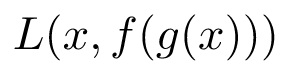
\includegraphics[width=0.25\textwidth]{images/ae_term.png} \\
    \vskip-5mm \\
    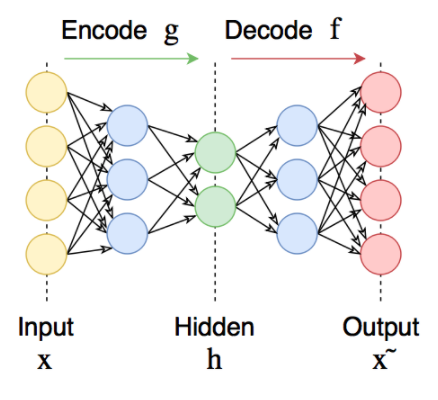
\includegraphics[width=0.55\textwidth]{images/ae.png}
\end{center}

\end{frame}
%-------------------------------------------------------------------------------
\begin{frame}
\frametitle{VAE}
\framesubtitle{Вариационный Автоэнкодер}

\begin{center}
    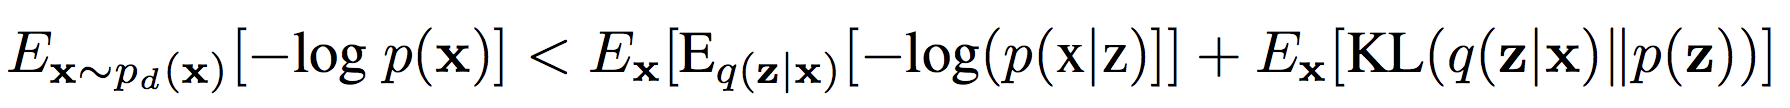
\includegraphics[width=0.8\textwidth]{images/elbo.png} \\
    \vskip-5mm \\
    \begin{columns}
        \begin{column}{0.5\textwidth}
            \begin{center}
                
\includegraphics[width=\textwidth]{images/vae_parts.png}
            \end{center}
        \end{column}
        \begin{column}{0.5\textwidth}
            \begin{center}
                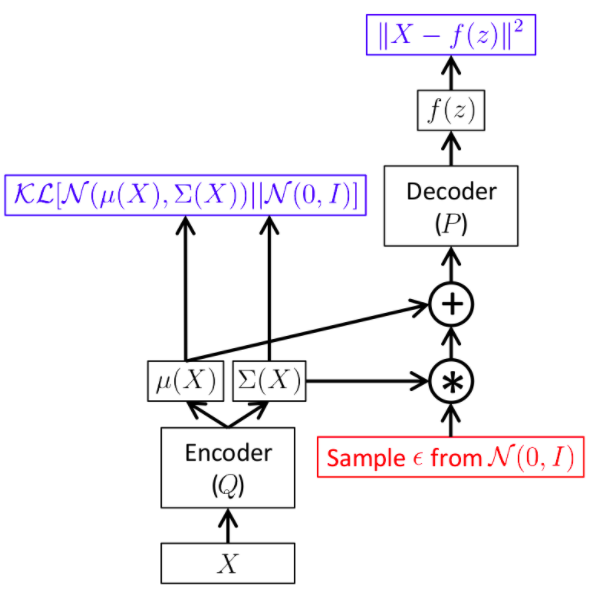
\includegraphics[width=\textwidth]{images/vae_terms.png}
            \end{center}
        \end{column}
    \end{columns}
    % 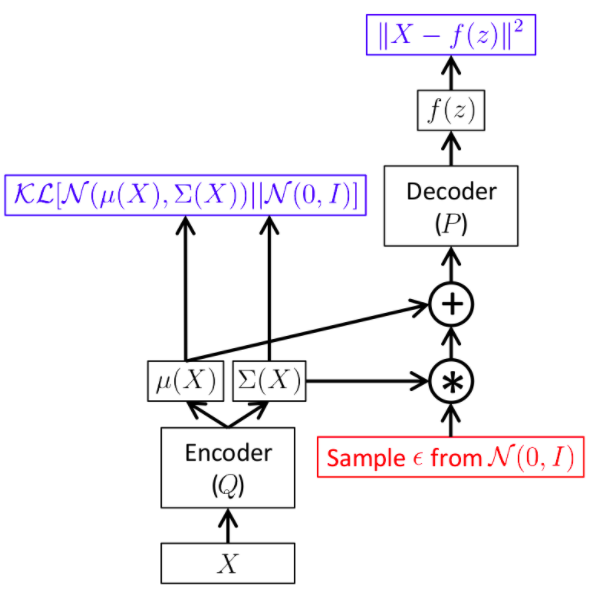
\includegraphics[width=0.5\textwidth]{images/vae_terms.png}
\end{center}

\end{frame}
%-------------------------------------------------------------------------------
\begin{frame}
\frametitle{VAE}
\framesubtitle{TextVAE (Bowman et al., 2016)}

\begin{center}
    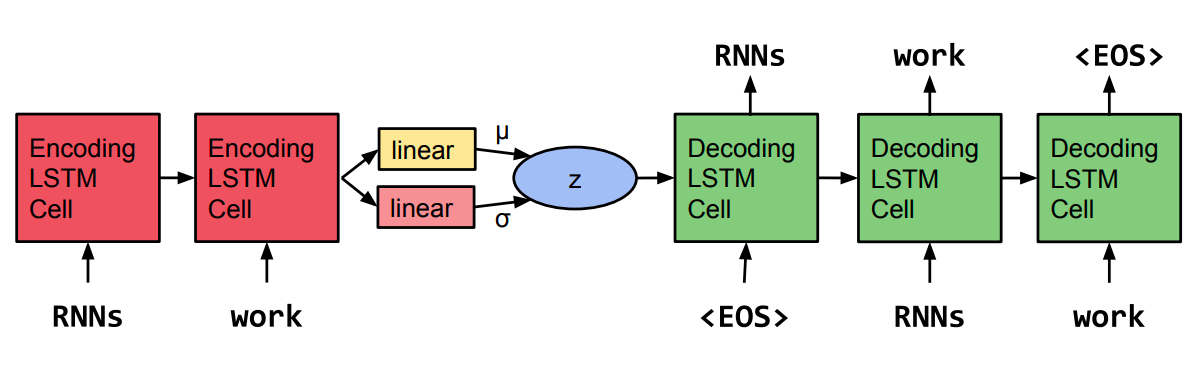
\includegraphics[width=0.5\textwidth]{images/text_vae.png}
\end{center}

Проблемы и решения:
\begin{itemize}
    \item Decoder начинает учиться быстрее encoder'a
    \begin{itemize}
        \item Дадим терму с KL переменный вес $w$, $w = 0 \Rightarrow 1$
        \item 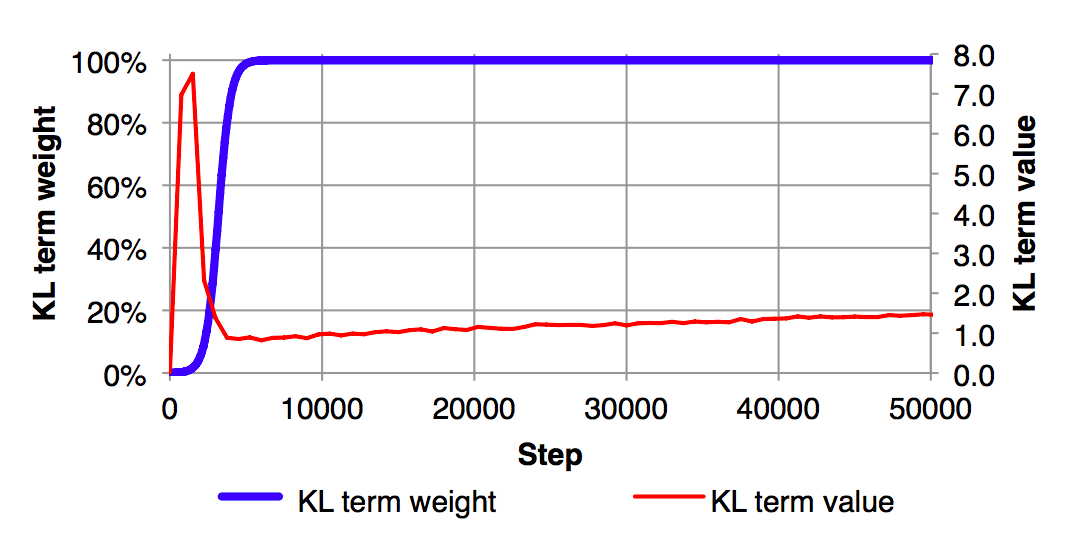
\includegraphics[width=0.45\textwidth]{images/kl_term_w.png}
    \end{itemize}
    \item Дополнительно портим жизнь энкодеру
    \begin{itemize}
        \item WordDropout: encoder'a случайно заменяем последнее слово на <UNK>
    \end{itemize}
\end{itemize}

\end{frame}
%-------------------------------------------------------------------------------
\begin{frame}
\frametitle{VAE}
\framesubtitle{Особенности TextVAE}

Путь между точками в латентном пространстве:
\begin{columns}[T]
    \begin{column}[T]{0.5\textwidth}
        \begin{center}
            AE \\
            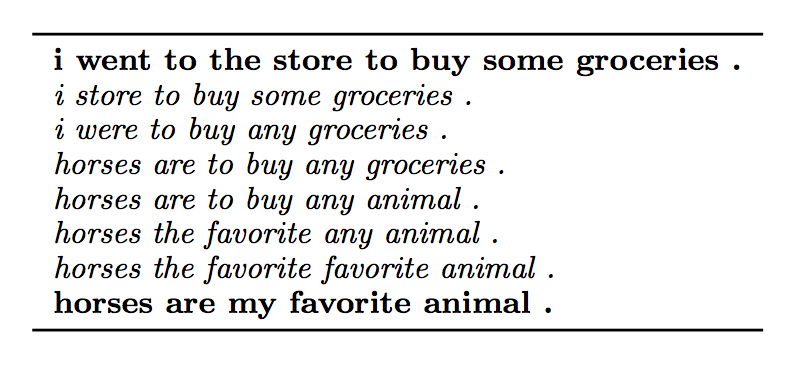
\includegraphics[width=1\textwidth]{images/ae_path.png}
        \end{center}
    \end{column}
    \begin{column}[T]{0.5\textwidth}
        \begin{center}
            VAE \\
            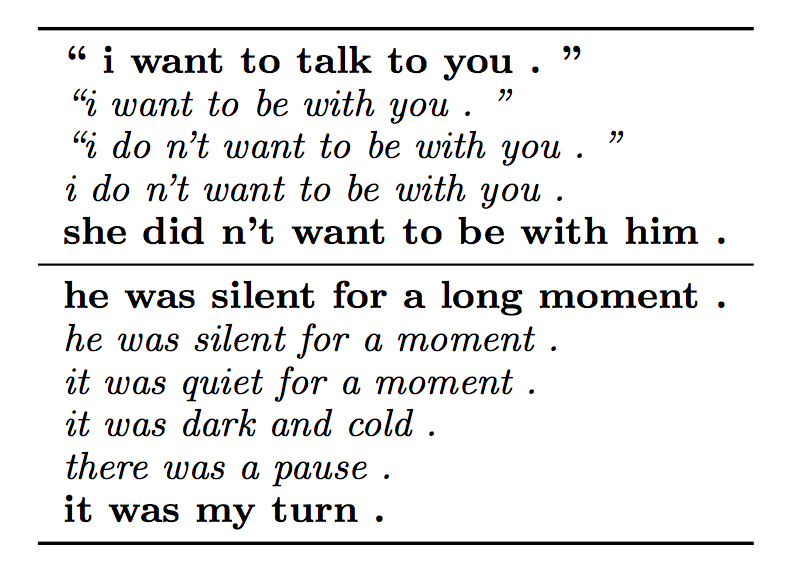
\includegraphics[width=1\textwidth]{images/vae_path.png}
        \end{center}
    \end{column}
\end{columns}

\end{frame}
%-------------------------------------------------------------------------------
\begin{frame}
\frametitle{VAE}
\framesubtitle{ConditionalVAE (Hu et al., 2018)}

\begin{center}
    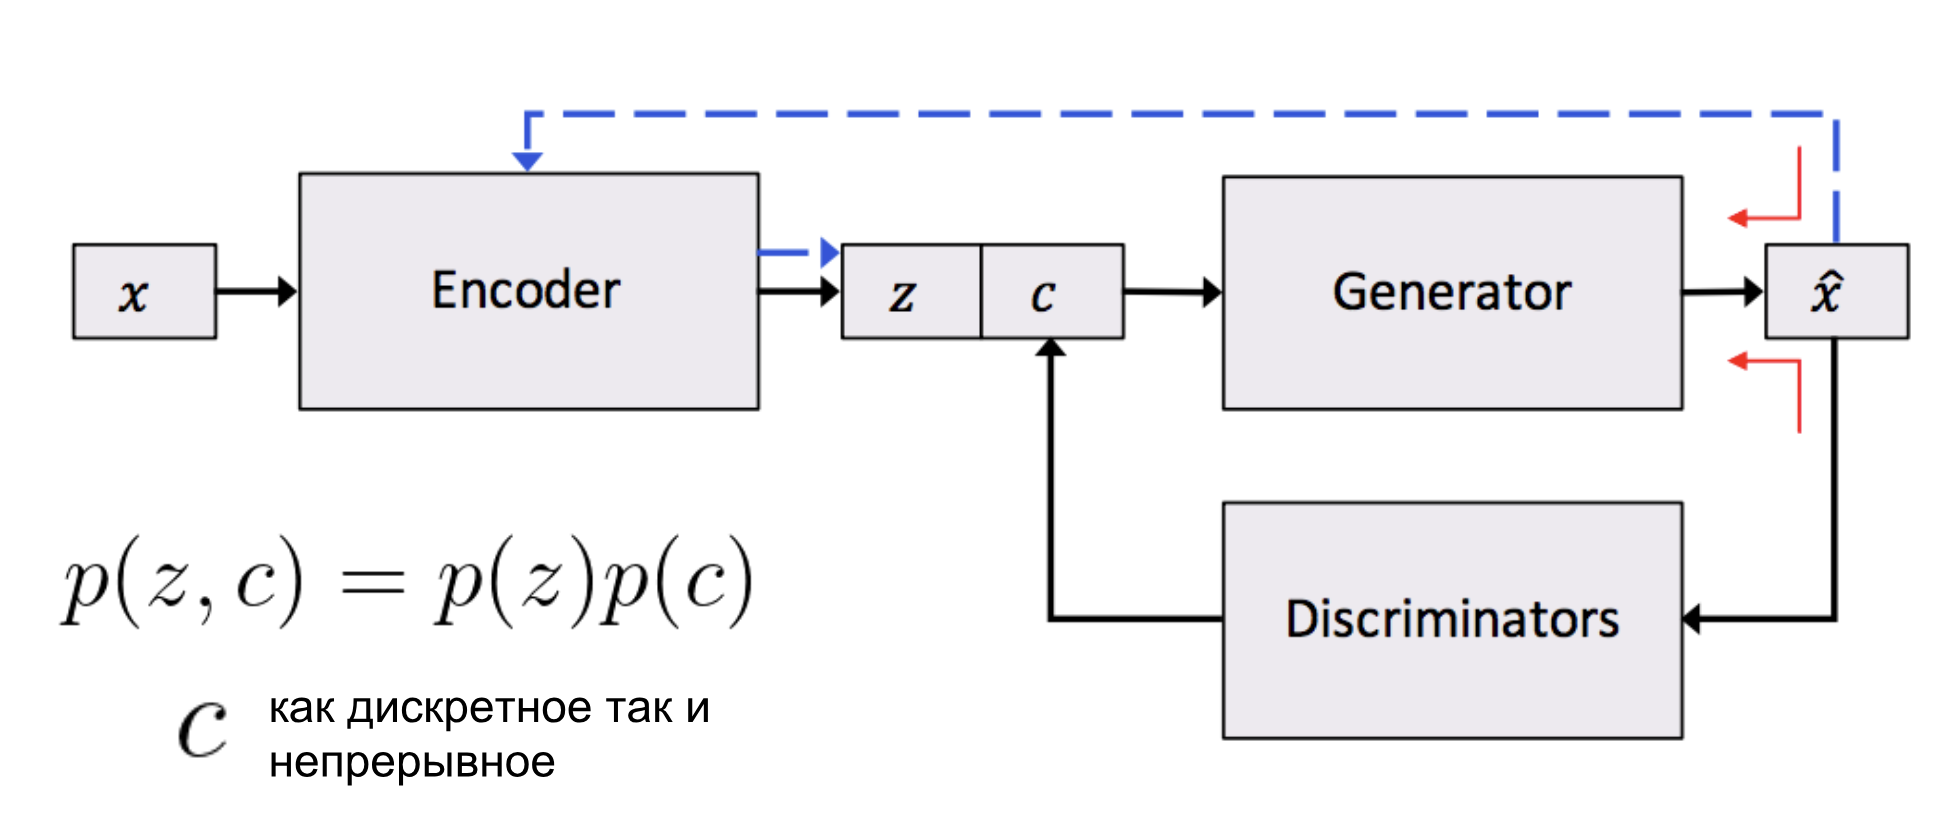
\includegraphics[width=0.8\textwidth]{images/cvae.png}
\end{center}
\begin{itemize}
    \item На каждое свойство свой дискриминатор
    \item $x$ не обязан иметь код при обучении - его можно получить из $p(c)$
    \item Нужно немного сэмплов
\end{itemize}

\end{frame}
%-------------------------------------------------------------------------------
\begin{frame}
\frametitle{VAE}
\framesubtitle{Лучшие подходы}

\begin{itemize}
    \item GRU => SRU
    \item 6 слоев, все дропауты по 0.3
    \begin{itemize}
        \item WordDropout
        \item LayerDropout
        \item RNNDropout
    \end{itemize}
    \item Быстрое сэмплирование с векторными операциями на GPU
    \begin{itemize}
        \item \~2x скорость обучения
    \end{itemize}
    \item Стохастический beam search с регулируемой температурой softmax-активации
    \begin{itemize}
        \item \~4x скорость сэмплирования
    \end{itemize}
    \item CNNEncoder (Zhang et al. 2016)
    \begin{itemize}
        \item 2, 3, 4, 5-граммы
        \item SELU-активация
    \end{itemize}
\end{itemize}

\end{frame}
%-------------------------------------------------------------------------------
\begin{frame}
\frametitle{VAE}
\framesubtitle{Self-Attention}

\begin{center}
    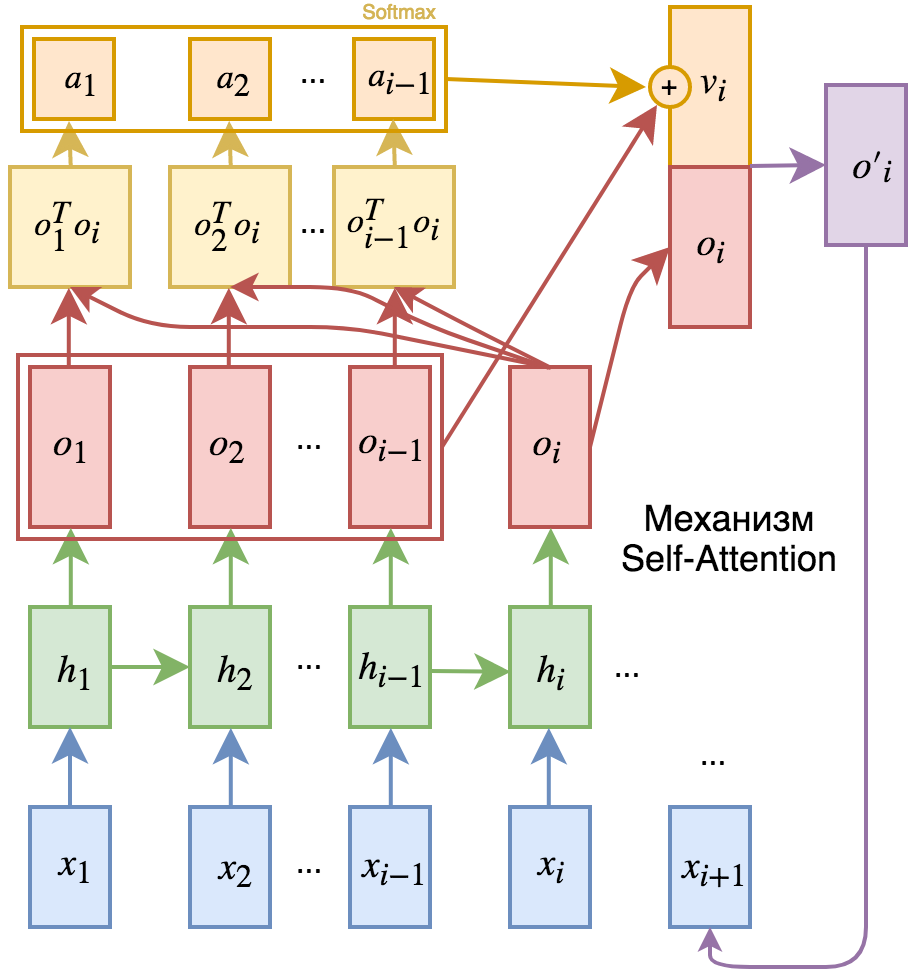
\includegraphics[width=0.57\textwidth]{images/self_attention.png}
\end{center}

\end{frame}
%-------------------------------------------------------------------------------
\begin{frame}
\frametitle{VAE}
\framesubtitle{Attention penalty}

\begin{center}
    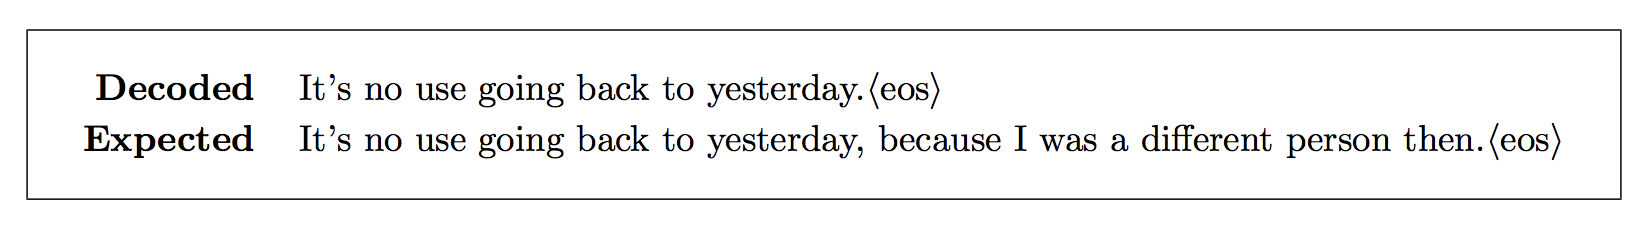
\includegraphics[width=0.8\textwidth]{images/bad_sample.png}
\end{center}

\vskip-6mm

\begin{columns}[T]
    \begin{column}[T]{0.5\textwidth}
        \begin{center}
            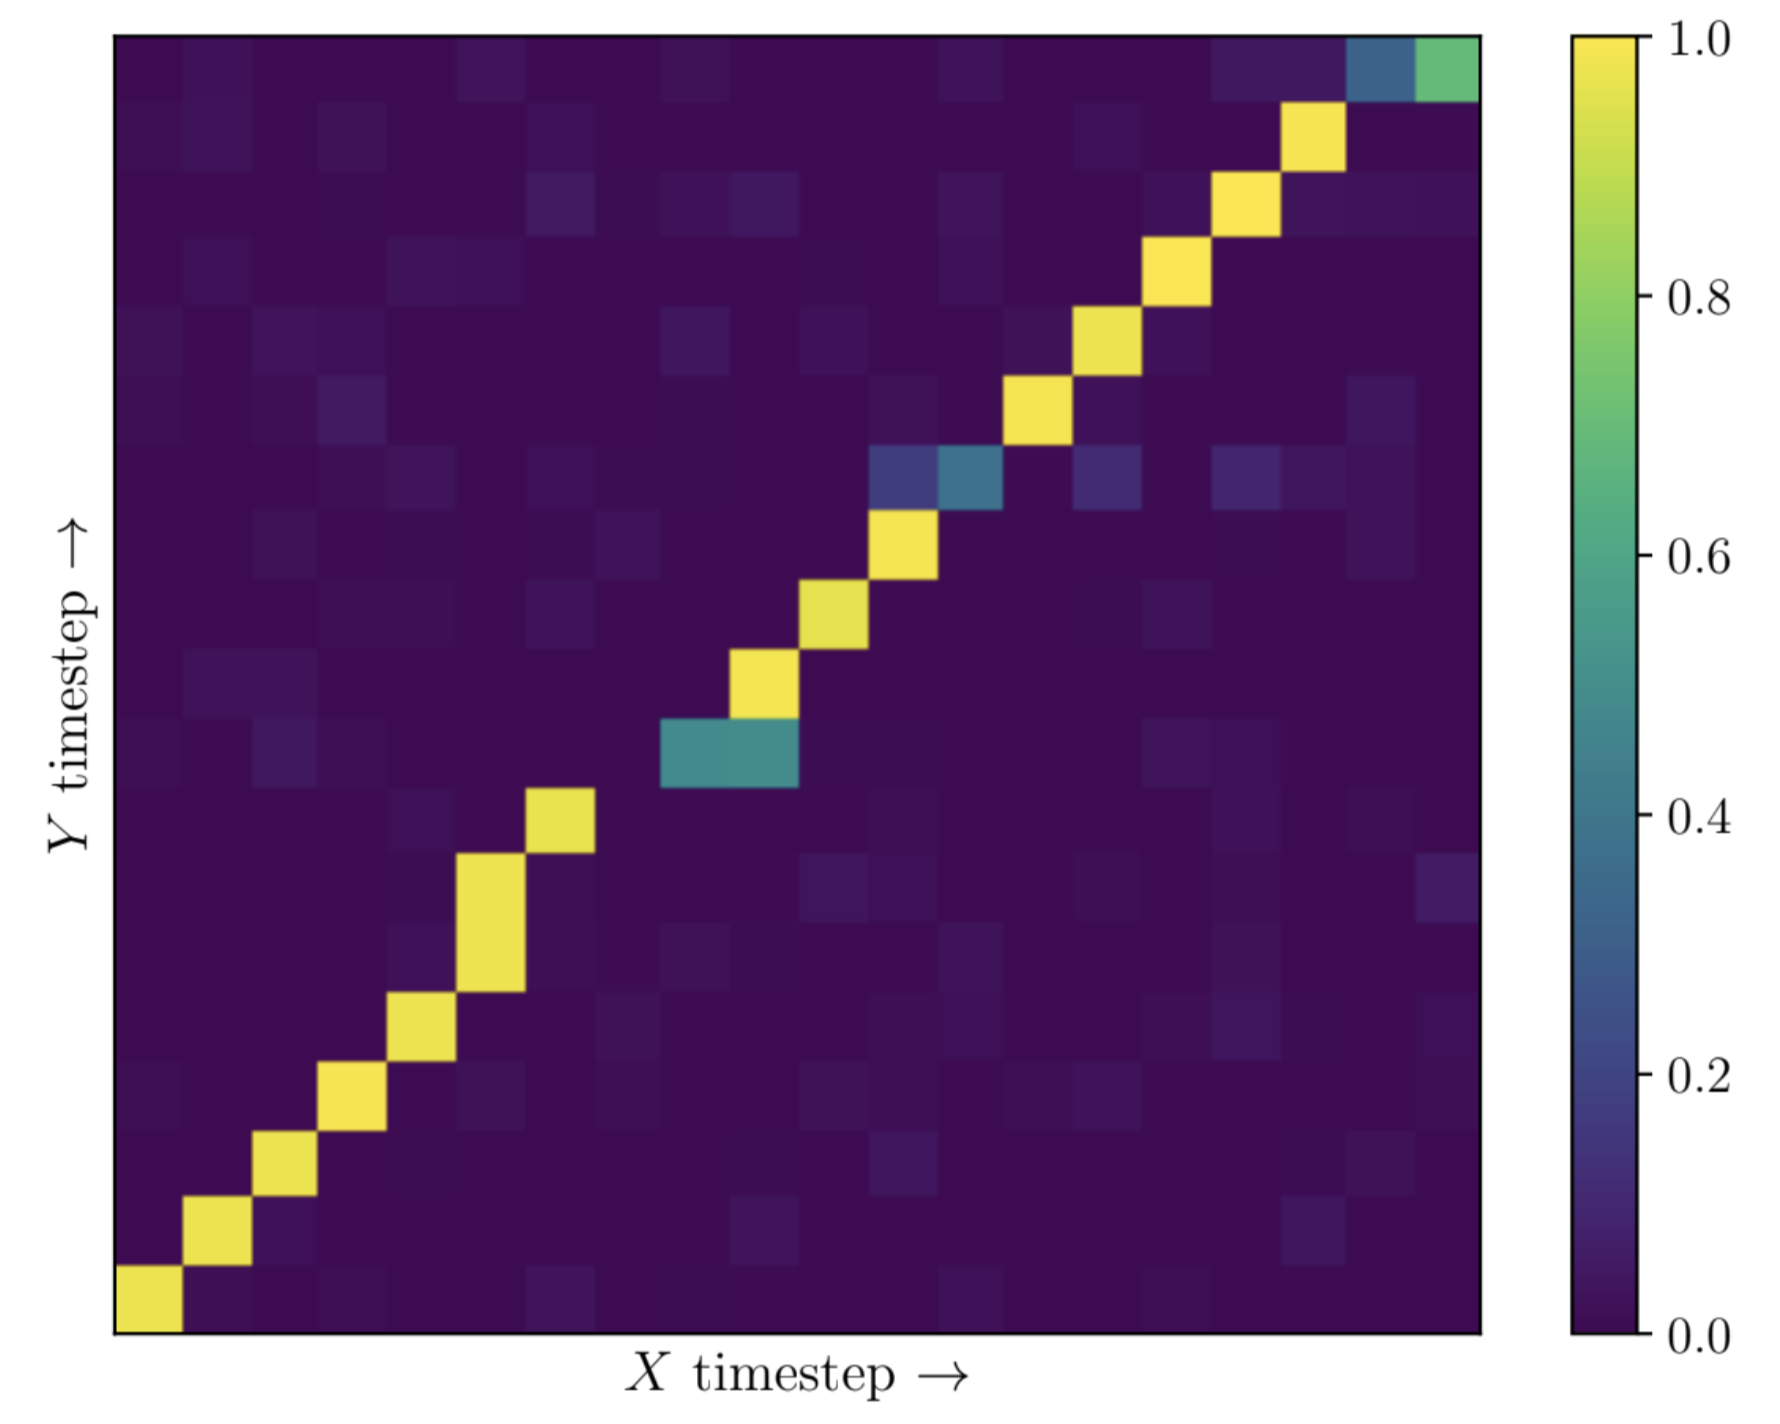
\includegraphics[width=0.9\textwidth]{images/attention.png}
        \end{center}
    \end{column}
    \begin{column}[T]{0.5\textwidth}
        \begin{center}
            Вывод может повторяться или быть недостаточно длинным, решение:
            \begin{itemize}
                \item Нормализация по длинне
                \item Бонус за длинных кандидатов $\beta \cdot |x|$
                \item Регуляризация по весам матрицы внимания
                $$cp(A) = \sum\limits_{j=1}^{|x|}{\log{\left[min(\sum\limits_{i=1}^{|x|}{a_{ij}}, 1)}\right]}$$
            \end{itemize}
        \end{center}
    \end{column}
\end{columns}

\end{frame}
%-------------------------------------------------------------------------------
\section{Результаты}
\begin{frame}
\frametitle{Результаты}
\framesubtitle{Сравнение моделей и подходов}

\begin{table}
\begin{tabular}{c | c c}
\toprule
\textbf{Test} & \textbf{CVAE} & \textbf{CVAE + SA} \\
\midrule
$X_{\texttt{gen}}$ & 83.483 & 84.263 \\
\bottomrule
\end{tabular}
\vskip-2mm
\caption{Точность на классификаторе}
\end{table}

\vskip-6mm

\begin{table}
\begin{tabular}{c | c c c c}
\toprule
\textbf{Test} & \textbf{VAE} & \textbf{CVAE} & \textbf{CVAE + SA} & \textbf{CVAE + SA + BS3 + CP} \\
\midrule
$X_{\texttt{test}}$ & \NaN & \NaN & 104 & 83 \\
\bottomrule
\end{tabular}
\vskip-2mm
\caption{Perplexity}
\end{table}

\vskip-6mm

\begin{table}
\begin{tabular}{c | c c c c}
\toprule
\textbf{Test} & \textbf{VAE} & \textbf{CVAE} & \textbf{CVAE + SA} & \textbf{CVAE + SA + BS3 + CP} \\
\midrule
$X_{\texttt{gen}}$ & 9.0 & 9.0 & 14.3 & 15.4 \\
\bottomrule
\end{tabular}
\vskip-2mm
\caption{BLEU * 100}
\end{table}

\vskip-6mm

\begin{table}
\begin{tabular}{c | c c c c}
\toprule
\textbf{Test} & \textbf{VAE} & \textbf{CVAE} & \textbf{CVAE + SA} & \textbf{CVAE + SA + BS3 + CP} \\
\midrule
$X_{\texttt{gen}}$ & 3.8 & 4.0 & 4.2 & 4.2 \\
\bottomrule
\end{tabular}
\vskip-2mm
\caption{Self-BLEU * 100}
\end{table}

\end{frame}
%-------------------------------------------------------------------------------
\begin{frame}
\frametitle{Результаты}
\framesubtitle{Выводы и будущая работа}

Выводы:
\begin{itemize}
    \item CVAE + Semi-supervised + декодэр на стероидах
    \item Анализ state-of-the-art методов генерации текста
    \item Анализ влияния данных на генерацию и способность выучить свойства
    \item Метрики и эмпирические проверки, позволяющие оценить сложность задачи
\end{itemize}

Будущая работа:
\begin{itemize}
    \item Попытаться проинтерпретировать важной свойств
    \begin{itemize}
        \item Латентное подпространство для $\Xtest \cap X$ из $VAE$
    \end{itemize}
    \item Акаковать проблему mode-collapsing'а в GAN'ах
    \begin{itemize}
        \item VAE => AAE
        \item $\alpha$-GAN
    \end{itemize}
\end{itemize}

\end{frame}
%-------------------------------------------------------------------------------
\section{Ссылки}
\begin{frame}
\frametitle{Ссылки}
\framesubtitle{Статьи, код и контакты}

\begin{enumerate}
    \item \begin{thebibliography}{99}
            \bibitem[Barone, 2017]{p1} Antonio Valerio Miceli Barone (2017)
            \newblock \href{https://arxiv.org/abs/1707.02275v1}{A parallel corpus of Python functions and documentation strings for automated code documentation and code generation}
        \end{thebibliography}
    \item Karpathy, Andrej (2015). \href{http://karpathy.github.io/2015/05/21/rnn-effectiveness/}{“The Unreasonable Effectiveness of Recurrent Neural Networks”.}
    \item \begin{thebibliography}{99}
            \bibitem[Bowman, 2016]{p1} Samuel R. Bowman (2016)
            \newblock \href{https://arxiv.org/abs/1511.06349}{Generating Sentences from a Continuous Space}
        \end{thebibliography}
    \item \begin{thebibliography}{99}
            \bibitem[Hu, 2018]{p1} Zhiting Hu (2018)
            \newblock \href{https://arxiv.org/abs/1703.00955}{Toward Controlled Generation of Text}
        \end{thebibliography}
    \item \begin{thebibliography}{99}
            \bibitem[Wang, 2017]{p1} Heng Wang (2017)
            \newblock \href{https://arxiv.org/abs/1712.00170}{Text Generation Based on Generative Adversarial Nets with Latent Variable}
        \end{thebibliography}
    \item \ULurl{https://github.com/stasbel/text-gen} (Генерация)
    \item \ULurl{https://github.com/stasbel/bachelor-thesis} (Презентация)
    \item \ULurl{https://t.me/stasbel}
\end{enumerate}

\end{frame}
%-------------------------------------------------------------------------------
%	END PRESENTATION SLIDES
%-------------------------------------------------------------------------------
\end{document}